\documentclass[a4paper,12pt]{article}
\usepackage[utf8]{inputenc}
\usepackage[english,russian]{babel}
\usepackage[T2A]{fontenc}
\usepackage{mathtext}
\usepackage{gauss}
\usepackage{graphicx}
\usepackage{amsmath, amsfonts, amssymb}
\newtheorem{theorem}{Теорема}
\usepackage[left=2.50cm, right=2.00cm, top=2.00cm, bottom=2.00cm]{geometry} 
\usepackage{mathdots} 
\usepackage[pdftex]{lscape}
\usepackage{mathtools}
\usepackage{pgfplots}
\pgfplotsset{compat=1.9}
\usepackage{graphicx}%Вставка картинок правильная
\usepackage{tikz}
\usepackage{float}%"Плавающие" картинки
 \usepackage{relsize}
\usepackage{wrapfig}%Обтекание фигур (таблиц, картинок и прочего)
\usepackage{ tipa }
\usepackage{amsmath}
  \usepackage[unicode=true, colorlinks=true, linkcolor=blue, urlcolor=blue]{hyperref}
\linespread{1}
\newcommand{\om}{\overline{o}}
\newcommand{\OB}{\underline{O}}
\newcommand{\eps}{\varepsilon}
\newcommand{\RR}{\mathbb{R}}
\newcommand{\NN}{\mathbb{N}}
\newcommand{\CC}{\mathbb{C}}
\newcommand{\QQ}{\mathbb{Q}}
\newcommand{\ZZ}{\mathbb{Z}}
\newcommand{\dx}{\d{dx}}
\newcommand{\ph}{\varphi}
\newcommand{\F}{\mathbb{F}}
\newcommand{\E}{\mathbb{E}}
\begin{document}	
	\begin{titlepage}
		
		
		\begin{center}
			\textsc{\textbf{МА-2, дз 1}}
		\end{center}
		
		\vspace{6em}
		
		
		
		\newbox{\lbox}
		\savebox{\lbox}{\hbox{Пупкин Иван Иванович}}
		\newlength{\maxl}
		\setlength{\maxl}{\wd\lbox}
		\hfill\parbox{11cm}{
			\hspace*{5cm}\hspace*{-5cm}Студент:\hfill\hbox to\maxl{Кондратьев Никита \hfill}\\
			\hspace*{5cm}\hspace*{-5cm}Группа:\hfill\hbox to\maxl{238}\\
		}
		
		
		
	\end{titlepage}
	\section*{1}
Привести двойной интеграл $\iint\limits_{D}f(x,y)dxdy$к повторному во всех возможнных порядках .
\begin{figure}[h]
	\centering
	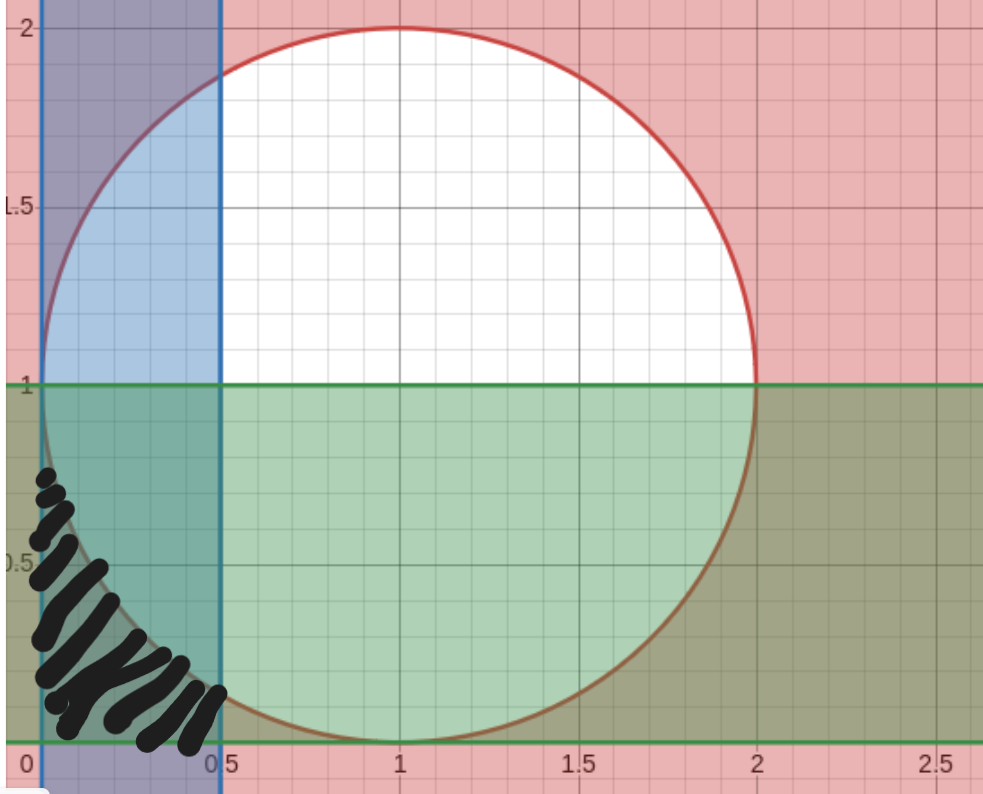
\includegraphics[width=0.5\textwidth]{Screenshot from 2024-09-23 11-34-24}
	\caption{Заштрихованная область - то что мы ищем}
	\label{fig:example}
\end{figure}

 \subsection*{(x,y)}
 		$$(y-1)^2 = 1-(x-1)^2$$
 		$$|y-1| =\sqrt{1-(x-1)^2} \text{ (раскроем с плюсом, т.к 1 четверть)}$$
 		$$y = 1+  \sqrt{1-(x-1)^2}$$
 		$$\int\limits_0^1dy\int\limits_{0}^{\sqrt{1-(y-1)^2}}fdx$$
 		
	 \subsection*{(y,x)}
	  		$$\int\limits_0^{\frac12}dx\int\limits_{0}^{\sqrt{1-(x-1)^2}}fdy$$
	  	\section*{2}
	  	Изменить порядок интегрированя в повторном интеграле. 
	  	$$\int\limits_{0}^{1}dy\int\limits_{\sqrt{4-4y}}^{\sqrt{4-y^2}} fdx+ \int\limits_{1}^{2}dy\int\limits_{0}^{\sqrt{4-y^2}} fdx$$
	  	\begin{figure}[h]
	  		\centering
	  		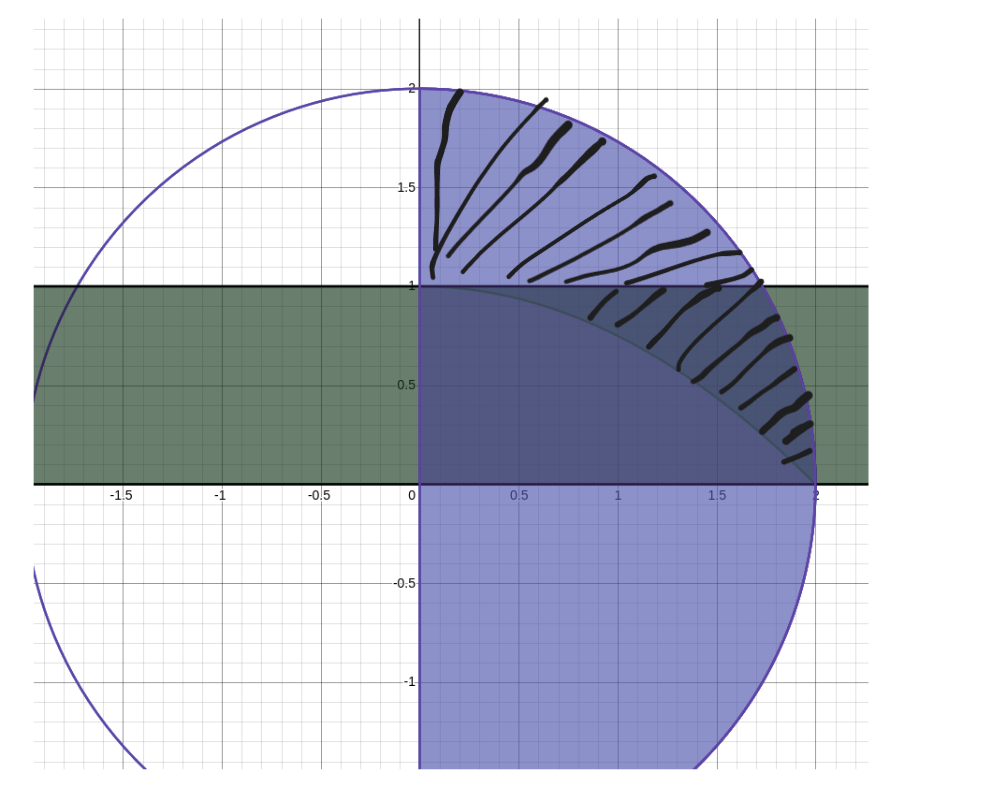
\includegraphics[width=0.5\textwidth]{Pasted image1}
	  		\caption{Заштрихованная область - то что мы ищем}
	  		\label{fig:example}
	  	\end{figure}
	  	Чтобы найти площадь этого куска можно сложить две части - верхнюю и нижнюю, но это муторно. А можно просто из четверти круга вычесть незаштрихованную часть. 
	  	$$\int\limits _0^2dx\int\limits_0^{\sqrt{4-x^2}}fdy - \int\limits _0^1dx\int\limits_0^{1-x^2/4}fdy$$
	  	\section*{3}
	  	Вычислить интеграл
	 $$\int\limits_0^2x^2dx\int\limits_{x}^{2}\ln(1+y^2)dy$$	
	 	  	\begin{figure}[h]
	 	\centering
	 	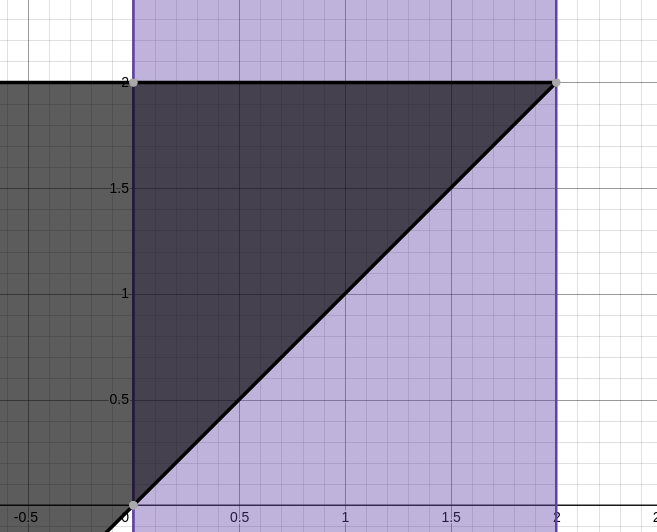
\includegraphics[width=0.5\textwidth]{Pasted image}
	 	\caption{Мы считаем вот этот треугольник }
	 	\label{fig:example}
	 \end{figure}
	 Чтобы было легче считать, поменяем порядок интгерирования. 
	 $$\int\limits_0^2x^2dy\int\limits_{y}^{2}\ln{(1+y^2)}dx =\int\limits_{0}^{2}\ln{(1+y^2)}dy\int\limits_{y}^{2}x^2dx $$
	 $$\int\limits_{y}^{2}x^2dx = \frac13\left(y^3-8\right)$$
	 $$\frac13\int\limits_{0}^{2}\ln{(1+y^2)}\cdot\left(y^3-8\right)dy$$
	 $$\text{(интегрируем по частям)  } \ln(1+y^2)(y^4/4-8y)|^2_0 -\frac14 \int\limits_{0}^{2}\left(\frac{2y}{1+y^2}\right)\cdot\left(y^2-2y\right) $$
	 $$= \frac13\cdot(-11\ln{5}-12-4\arcctg2)$$
\end{document}